%%%%%%%%%%%%%%%%%%%%%%%%%%%%%%%%%%%%%%%%%%  不使用 authblk 包制作标题  %%%%%%%%%%%%%%%%%%%%%%%%%%%%%%%%%%%%%%%%%%%%%%
%-------------------------------PPT Title-------------------------------------
\title{19-多体相互作用理论}
%-----------------------------------------------------------------------------
%----------------------------Author & Date------------------------------------

%\author[\textrm{Jun\_Jiang}]{姜\;\;骏\inst{}} %[]{} (optional, use only with lots of authors)
%% - Give the names in the same order as the appear in the paper.
%% - Use the \inst{?} command only if the authors have different
%%   affiliation.
%\institute[BCC]{\inst{}%
\institute[Gain~Strong]{\inst{}%
%\vskip -20pt 北京市计算中心}
\vskip -20pt {\large 格致斯创~科技}}
\date[\today] % (optional, should be abbreviation of conference name)
{%	{\fontsize{6.2pt}{4.2pt}\selectfont{\textcolor{blue}{E-mail:~}\url{jiangjun@bcc.ac.cn}}}
\vskip 45 pt {\fontsize{8.2pt}{6.2pt}\selectfont{%清华大学\;\;物理系% 报告地点
	\vskip 5 pt \textrm{2023.04.22}}}
}

%% - Either use conference name or its abbreviation
%% - Not really information to the audience, more for people (including
%%   yourself) who are reading the slides onlin%%   yourself) who are reading the slides onlin%%   yourself) who are reading the slides onlineee
%%%%%%%%%%%%%%%%%%%%%%%%%%%%%%%%%%%%%%%%%%%%%%%%%%%%%%%%%%%%%%%%%%%%%%%%%%%%%%%%%%%%%%%%%%%%%%%%%%%%%%%%%%%%%%%%%%%%%

\subject{}
% This is only inserted into the PDF information catalog. Can be left
% out.
%\maketitle
\frame
{
%	\frametitle{\fontsize{9.5pt}{5.2pt}\selectfont{\textcolor{orange}{“高通量并发式材料计算算法与软件”年度检查}}}
\titlepage
}
%-----------------------------------------------------------------------------

%------------------------------------------------------------------------------列出全文 outline ---------------------------------------------------------------------------------
%\section*{}
%\frame[allowframebreaks]
%{
%  \frametitle{Outline}
%%  \frametitle{\textcolor{mycolor}{\secname}}
%  \tableofcontents%[current,currentsection,currentsubsection]
%}
%%在每个section之前列出全部Outline
%%类似的在每个subsection之前列出全部Outline是\AtBeginSubsection[]
%\AtBeginSection[]
%{
%  \frame<handout:0>%[allowframebreaks]
%  {
%    \frametitle{Outline}
%%全部Outline中,本部分加亮
%    \tableofcontents[current,currentsection]
%  }
%}

%-----------------------------------------------PPT main Body------------------------------------------------------------------------------------
\small
%\section{\rm{VASP~}软件中\rm{PAW~}计算的实现}
%\frame
%
%	\frametitle{\textrm{VASP}计算的特色}
%	相比于与普通的第一原理计算软件,\textrm{VASP}很好地平衡了计算效率和精度的问题,总的来说,\textrm{VASP}主要通过这几个特色保证了计算的高效能
%	\begin{itemize}
%	     \item 迭代与优化算法的多样性\\
%		     本质上电荷密度迭代 \textrm{\&\&} 体系总能量优化是相同的优化问题,采用了类似的算法\upcite{CMS6-15_1996,PRB54-11169_1996}:\\
%			\textcolor{blue}{\textrm{Pseudo-Newton、Conjugate-Gradient、Broyden~mix、damping-factor、RMM-DIIS}}
%	     \item 尽可能采用局域基(原子轨道基)函数:~\\
%		     \textcolor{blue}{\textrm{LREAL}}=\textcolor{red}{\textrm{.TRUE.}}\\
%			优化的投影函数也尽可能在实空间表示
%	     \item \textrm{PAW}原子数据集:\textcolor{blue}{优异的赝势}\upcite{PRB59-1758_1999}
%	\end{itemize}
%}
\section{电子相关与多体理论}
\frame
{
	\frametitle{\textrm{Green's function}}
	\begin{itemize}
		\item 时间序列的\textrm{Green's function}定义为$G(\vec r_1,t_1;\vec r_2,t_2)=-\mathrm{i}\langle\Theta_0^N|\hat{\mathbf{T}}[\hat\psi(\vec r_1,t_1)\hat\psi^{\dag}(\vec r_2,t_2)]|\Theta_0^N\rangle$
		\item \textrm{Green function}的\textrm{Lehmann}表象为$$G(\vec r_1,\vec r_2;\omega)=\sum\limits_i\dfrac{\Psi_i(\vec r_1)\Psi_i^{\dag}(\vec r_2)}{\omega-\varepsilon_i+\mathrm{i}\eta\mathrm{sign}(\varepsilon_i-\mu)}\qquad\eta\rightarrow0^+$$
			由于频率域中时间序列的\textrm{Green's function}包含$(N-1)$个粒子和$(N+1)$个粒子体系的全部激发谱,它们与\textrm{Green's function}在复平面的极值对应
	\end{itemize}
\begin{figure}[h!]
\centering
\vspace{-5pt}
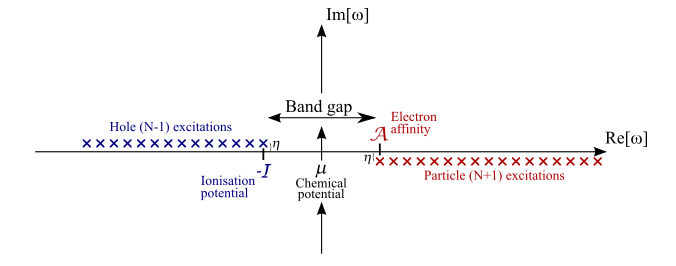
\includegraphics[height=0.80in,width=2.05in,viewport=30 1 660 265,clip]{Figures/GW-0.png}
\caption{\textrm{\small{The poles of the time-ordered Green's function.}}}%(与文献\cite{EPJB33-47_2003}图1对比)
\label{GW-0}
\end{figure}
}

\frame
{
	\frametitle{\textrm{Green's function}与\textrm{Hamiltonian}}
	\begin{itemize}
		\item \textrm{Green's function}是\textrm{Hamiltonian}的\textcolor{blue}{翻转}
			\begin{displaymath}
				1=(\omega-H)G\Longleftrightarrow G^{-1}=(\omega -H)
			\end{displaymath}
		\item \textrm{Lehmann}表象下,\textrm{Kohn-Sham}(无相互作用的)\textrm{Hamiltonian}对应的\textrm{Green' function}
			\begin{displaymath}
				G_{\textcolor{magenta}{0}}(\vec r,\vec r^{\prime};\omega)=\sum_n\dfrac{\psi_n(\vec r)\psi_n^{\ast}(\vec r^{\prime})}{\omega-\varepsilon_n+\mathrm{i}\eta\mathrm{sign}(\varepsilon_n-\mu)}
			\end{displaymath}
		\item 相互作用\textrm{Hamiltonian}的\textrm{Green's function}
		\fontsize{9.5pt}{4.2pt}\selectfont{	\begin{displaymath}
			\hspace*{-35pt}	\begin{aligned}
				&\underbrace{\bigg(-\dfrac{\hbar^2}{2m_e}\nabla^2+V_{\mathrm{ion}}(\vec r)+V_H(r)\bigg)}+\Sigma(\vec r,\vec r^{\prime},\omega)=H(\omega)\Longrightarrow H_0+\Sigma(\textcolor{red}{\omega})=H(\textcolor{red}{\omega})\\
					&\quad\qquad\qquad\mathrm{\textcolor{blue}{non-int.}} %\mathrm{energy/frequency dependent Hamiltonian}
				\end{aligned}
			\end{displaymath}}
	\end{itemize}
}

\frame
{
	\frametitle{多重散射与\textrm{Green's function}}
	\vspace{-0.2in}
\begin{displaymath}
	\begin{aligned}
		(H_0-\omega)+\Sigma(\omega)&=(H-\omega)\\
		-G_0^{-1}(\omega)+\Sigma(\omega)&=-G^{-1}-\omega)\\
		G^{-1}(\omega)&=G_0^{-1}-\omega)-\Sigma(\omega)
	\end{aligned}
\end{displaymath}
\begin{figure}[h!]
	\vspace{-0.52in}
\centering
%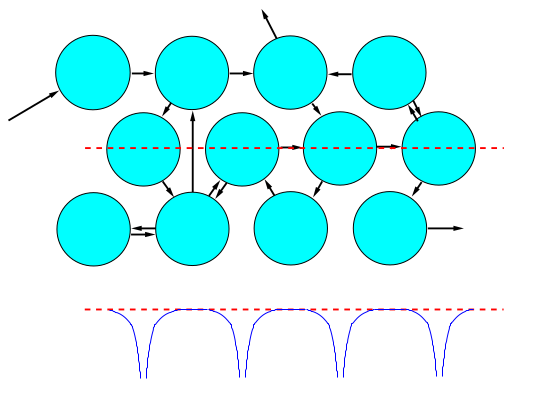
\includegraphics[height=1.80in,width=1.95in,viewport=5 0 515 495,clip]{Figures/multiple-scattering_theory.png}
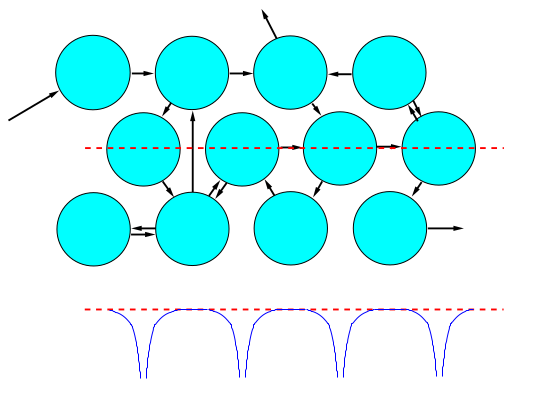
\includegraphics[height=2.30in,width=2.44in,viewport=5 0 515 495,clip]{Figures/multiple-scattering_theory.png}
\caption{\tiny \textrm{Central idea of multiple scattering theory:~ decomposition of electronic motion into scattering at atomic sites and free-electron like propagation in between. The bottom of the figure gives a sketch for the potential along the dashed line.}}
\label{Multi-scattering}
\end{figure}
}

\frame
{
	\frametitle{多重散射与\textrm{Green's function}}
\begin{figure}[h!]
	\vspace{-5pt}
\centering
\animategraphics[autoplay, loop, height=1.2in]{1}{Figures/Multi_scattering-}{0}{9}
\label{Multiple_scattering-0-9}
\end{figure}
\textcolor{blue}{多重散射:~}入射波是\textcolor{red}{所有来自其他散射中心的出射波叠加}
			\begin{displaymath}
				\begin{aligned}
					\tilde G=&\tilde G_0+G_0\mathbf{t}\tilde G_0+G_0\mathbf{t}\tilde G_0\mathbf{t}\tilde G_0+\cdots\\
					=&\tilde G_0+\tilde G_0\mathbf{t}\tilde G \Longrightarrow \tilde G=(\tilde G_0^{-1}-\mathbf{t})^{-1}
%					\tilde G=&(\tilde G_0^{-1}-\mathbf{t})^{-1}
				\end{aligned}
			\end{displaymath}
}

\frame
{
	\frametitle{\textrm{Green function}与自能}
	\textrm{Dyson}方程
	\begin{displaymath}
		\begin{aligned}
	&G(\vec r_1,t_1;\vec r_2,t_2)=G_0(\vec r_1,t_1;\vec r_2,t_2)\\
	&+\int G_0(\vec r_1,t_1;\vec r_3,t_3)\Sigma(\vec r_3,t_3;\vec r_4,t_4)G(\vec r_4,t_4;\vec r_2,t_2)\mathrm{d}t_3\mathrm{d}\vec r_3\mathrm{d}t_4\mathrm{d}\vec r_4
		\end{aligned}
	\end{displaymath}
	\begin{itemize}
		\item \textrm{Dyson}方程描述了相互作用体系$G$通过自能$\Sigma$与近独立体系(传播子)$G_0$关联,自能$\Sigma$是非局域,非\textrm{Hermitian},并与时间相关
		\item 通过求解含有自能$\Sigma$的准粒子方程,可以求解得到多体体系中重整化电子的量子态(\textrm{Hedin}方程)
			$$\bigg[\hat h_0(\vec r_1)+v_H(\vec r_1)\bigg]\Psi(\vec r_1)+\int\Sigma(\vec r_1,\vec r_2;\omega^{\mathrm{QP}})\Psi(\vec r_2)\mathrm{d}\vec r_2=\varepsilon^{\mathrm{QP}}\Psi(\vec r_1)$$
	\end{itemize}
}

\frame
{
	\frametitle{\textrm{Green's function}的物理意义}
	时间序列的\textrm{Green's function}$G(\vec r,\vec r^{\prime},t-t^{\prime})$描述了粒子由$(\vec r,t)$到$\vec r^{\prime},t^{\prime}$的传播\footnote{\fontsize{6.5pt}{4.2pt}\selectfont{因此\textrm{Green's funtion}被称为传播子.}}:~换言之,假设粒子在时空点$(\vec r,t)$位置出现,则$G(\vec r,\vec r^{\prime},t-t^{\prime})$表示在时空点$(\vec r^{\prime},t^{\prime})$找到粒子的概率
	\begin{displaymath}
		G_{0}(\vec r,\vec r^{\prime};\omega)=\sum_n^{\mathrm{all}}\dfrac{\psi_n^{\ast}(\vec r)\psi_n(\vec r^{\prime})}{\omega-\varepsilon_n+\mathrm{i}\eta\mathrm{sign}(\varepsilon_n-\mu)}
	\end{displaymath}
\begin{figure}[h!]
	\vspace{-0.52in}
\centering
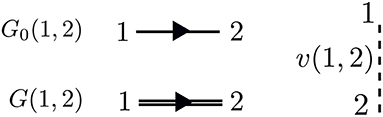
\includegraphics[height=0.50in,width=1.44in,viewport=0 0 315 125,clip]{Figures/DFT_GW-3.jpg}
%\caption{\tiny \textrm{Central idea of multiple scattering theory:~ decomposition of electronic motion into scattering at atomic sites and free-electron like propagation in between. The bottom of the figure gives a sketch for the potential along the dashed line.}}
\label{Green's_function-physical interpretation}
\end{figure}
\fontsize{7.5pt}{4.2pt}\selectfont{
	\begin{itemize}
		\item 粒子传播子:$G_0(1,2)=G_0(\vec r_1,\vec r_2,t_2-t_1)$且\textcolor{blue}{$(t_2>t_1)$}
			\begin{displaymath}
				G_0(1,2)=\sum_n^{\textcolor{blue}{\mathrm{vir.}}}\psi_n^{\ast}(\vec r_1)\psi_n(\vec r_2)\mathrm{e}^{-\mathrm{i}(\varepsilon_n-\mu)(\textcolor{blue}{t_2-t_1})}
			\end{displaymath}
		\item 孔传播子:$G_0(1,2)=G_0(\vec r_1,\vec r_2,t_2-t_1)$且\textcolor{blue}{$(t_1>t_2)$}
			\begin{displaymath}
				G_0(1,2)=\sum_n^{\textcolor{blue}{\mathrm{occ.}}}\psi_n^{\ast}(\vec r_1)\psi_n(\vec r_2)\mathrm{e}^{-\mathrm{i}(\varepsilon_n-\mu)(\textcolor{blue}{t_1-t_2})}
			\end{displaymath}
	\end{itemize}}
}

\frame
{
	\frametitle{\textrm{Hedin}方程的求解} 
	\textrm{Hedin}方程是积分-微分,可以通过迭代求解
\begin{figure}[h!]
\centering
\vspace{-10pt}
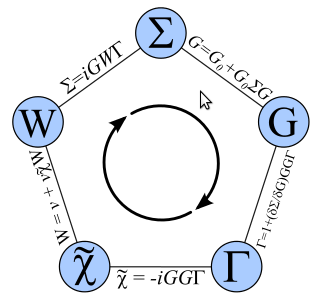
\includegraphics[height=1.0in,width=1.05in,viewport=5 5 330 335,clip]{Figures/GW-1.png}
%\caption{\textrm{\small{The relation of the varibous Green's function.}}}%(与文献\cite{EPJB33-47_2003}图1对比)
\label{GW-1}
\end{figure}
	\begin{itemize}
			\vspace{-15pt}
		\item 定义不可约极化率$\tilde\chi$,$\tilde\chi(\vec r_1,t_1;\vec r_2,t_2)\equiv\dfrac{\delta n(\vec r_1,t_1)}{\delta U_{e\!f\!f}(\vec r_2,t_2)}=-\mathrm{i}\dfrac{\delta G(\vec r_1,t_1,\vec r_1,t_1+\eta)_{\eta\rightarrow0}}{\delta U_{e\!f\!f}(\vec r_2,t_2)}$
		\item 定义动态屏蔽相互作用$W(\vec r_1,t_1;\vec r_2,t_2)\equiv\int\epsilon^{-1}(\vec r_1,t_1;\vec r_3,t_3)v(\vec r_3,r_3;\vec r_2,t_2)\mathrm{d}t_3\mathrm{d}\vec r_3$
		\item 介电矩阵与不可约极化率满足关系:
			\begin{displaymath}
				\begin{aligned}
					&\epsilon(\vec r_1,t_1;\vec r_2,t_2)\\
					=&\delta(\vec r_1,t_1;\vec r_2,t_2)-\int v(\vec r_,t_1,\vec r_3,t_3)\tilde\chi(\vec r_3,t_3;\vec r_2,t_2)\mathrm{d}t_3\mathrm{d}\vec r_3
				\end{aligned}
			\end{displaymath}
	\end{itemize}

}

\frame
{
	\frametitle{$GW$近似}
	直接求解\textrm{Hedin}方程是非常复杂的,有必要采取近似(把\textrm{vertex}函数用局域瞬时函数替代),这就是$GW$近似
	$$\Gamma(\vec r_{12},t_{12};\vec r_3t_3)\approx\delta(\vec r_1,t_1;\vec r_2,t_2)\delta(\vec r_1,t_1;\vec r_3,t_3)\equiv\Gamma^{GW}(\vec r_{12},t_{12};\vec r_3,r_3)$$
\begin{figure}[h!]
\centering
\vspace{-15pt}
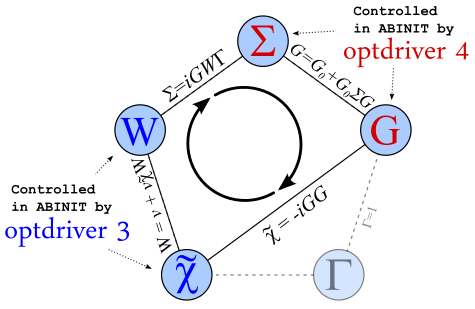
\includegraphics[height=1.0in,width=1.65in,viewport=5 5 530 320,clip]{Figures/GW-3.png}
%\caption{\textrm{\small{The relation of the varibous Green's function.}}}%(与文献\cite{EPJB33-47_2003}图1对比)
\label{GW-2}
\end{figure}
频率空间内,$GW$近似的自能表示为
$$\Sigma(\vec r_1,\vec r_2;\omega)=\dfrac{\mathrm i}{2\pi}\int \mathrm e^{\mathrm i\omega^{\prime}\delta^+}G(\vec r_1,\vec r_2;\omega+\omega^{\prime})W(\vec r_1,\vec r_2;\omega^{\prime})\mathrm{d}\omega^{\prime}$$
}

\frame
{
	\frametitle{由$GW$到$G_0W_0$近似}
	自洽迭代的$GW$方程求解仍然非常复杂,通常选择足够好的近似的$G$和$W$,作单次计算(即$G_0W_0$近似)得到自能
	$$\Sigma(\vec r_1,t_1;\vec r_2,t_2)=\mathrm{i}G_0^{\mathrm{KS}}W_0(\vec r_1,t_1+\eta;\vec r_2,t_2)_{\eta\rightarrow0}$$
	这里$G_0^{\mathrm{KS}}$由独立粒子的\textrm{Kohn-Sham(KS)}Hamiltonian

	屏蔽相互作用由\textrm{KS}本征态能量和波函数的\textrm{RPA}计算的到
	$$\chi^0(\vec r_1,t_1;\vec r_2,t_2)=-\mathrm{i}G_0^{\mathrm{KS}}(\vec r_1,t_1;\vec r_2,t_2)G_0^{\mathrm{KS}}(\vec r_1,t_1;\vec r_2,t_2)$$
	当准粒子波函数用\textrm{KS}轨道近似,本征态$\varepsilon^{\mathrm{KS}}$附近的准粒子能量$\varepsilon^{\mathrm{QP}}$用自能展开
	$$\varepsilon^{\mathrm{QP}}=\varepsilon^{\mathrm{KS}}+Z\langle\Psi^{\mathrm{KS}}|\Sigma(\varepsilon^{\mathrm{KS}}-v_{\mathrm{XC}})|\Psi^{\mathrm{KS}}\rangle$$
	这里重整化因子$Z$定义为$$Z\equiv\bigg[1-\langle\Psi^{\mathrm{KS}}\bigg|\dfrac{\partial\Sigma(\varepsilon)}{\partial\varepsilon^{\mathrm{KS}}}\bigg|\Psi^{\mathrm{KS}}\rangle\bigg]^{-1}$$
}

\frame
{
	\frametitle{$GWA$与\textrm{LDA+}$U$}
	\begin{displaymath}
		\begin{aligned}
			V_{m\sigma}^{GWA}=&\sum_{m^{\prime}\sigma^{\prime}}U_{mm^{\prime}}^0n_{m^{\prime}\sigma^{\prime}}-U_{mm}^0n_{m\sigma}-\sum_{m^{\prime}\neq m}J_{mm^{\prime}}n_{m^{\prime}\sigma}\\
			+&\left( \frac12-n_{m\sigma} \right)\sum_{m^{\prime}}W_{mm^{\prime}}
		\end{aligned}
	\end{displaymath}
	其中$U_{mm^{\prime}}^0$是\textcolor{blue}{未屏蔽\textrm{Coulomb~}相互作用矩阵},$J_{mm^{\prime}}$是\textcolor{blue}{交换矩阵}\\
	$W_{mm^{\prime}}$是\textcolor{red}{电子相关作用的矩阵$W_{\mathrm c}(\vec r,\vec r^{\prime};0)$的矩阵元}

	定义屏蔽相互作用参数$W$
	\begin{displaymath}
		W=-\sum_{m^{\prime}}W_{mm^{\prime}}
	\end{displaymath}
	因此,$\mathrm{GWA}$近似的矩阵元表示为
	\begin{displaymath}
			V_{m\sigma}^{GWA}=\sum_{m^{\prime}\sigma^{\prime}}U_{mm^{\prime}}^0n_{m^{\prime}\sigma^{\prime}}-(U_{mm}^0-W)n_{m\sigma}-\sum_{m^{\prime}\neq m}J_{mm^{\prime}}n_{m^{\prime}\sigma}-\frac12W
	\end{displaymath}
}

\frame
{
	\frametitle{$GWA$与\textrm{LDA+}$U$}
	对应于\textrm{LSDA},势能的修正
	\begin{displaymath}
		\begin{aligned}
			\delta V_{m\sigma}=&V_{m\sigma}^{GWA}-V_{m\sigma}^{\mathrm{LSDA}}\\
			=&\sum_{m^{\prime}\sigma^{\prime}}U_{mm^{\prime}}^0n_{m^{\prime}\sigma^{\prime}}-(U_{mm^{\prime}}^0-W)n_{m\sigma}-\sum_{m^{\prime}\neq m}J_{mm^{\prime}}n_{m^{\prime}\sigma}-\frac12W\\
			-&F^0\sum_{m^{\prime}\sigma^{\prime}}n_{m^{\prime}\sigma^{\prime}}+J\sum_mn_{m\sigma}+\frac12(F^0-J)\\
			=&\sum_{m^{\prime}\sigma^{\prime}}(U_{mm^{\prime}}^0-F^0)n_{m^{\prime}\sigma^{\prime}}-(U_{mm^{\prime}}^0-W)n_{m\sigma}-\sum_{m^{\prime}\neq m}J_{mm^{\prime}}n_{m^{\prime}\sigma}\\
			-&\frac12W+J\sum_mn_{m\sigma}+\frac12(F^0-J)
		\end{aligned}
	\end{displaymath}
}

\frame
{
	\frametitle{$GWA$与\textrm{LDA+}$U$}
	\textcolor{red}{注意:~}$U_{mm^{\prime}}^0-F^0$只与\textrm{Slater~}函数$F^k(k\neq0)$有关,与$F^0$无关,并且
	\begin{displaymath}
		U_{mm^{\prime}}^0-F^0=U_{mm^{\prime}}-U
	\end{displaymath}
	这里$U=F^0-W$是屏蔽\textrm{Coulomb~}参数,$U_{mm^{\prime}}$是屏蔽\textrm{Coulomb~}矩阵
	\begin{displaymath}
		\begin{aligned}
			\delta V_{m\sigma}=&V_{m\sigma}^{GWA}-V_{m\sigma}^{\mathrm{LSDA}}\\
			=&\sum_{m^{\prime}\sigma^{\prime}}U_{mm^{\prime}}n_{m^{\prime}-\sigma}+\sum_{m^{\prime}\neq m}(U_{mm^{\prime}}-J_{mm^{\prime}})n_{m^{\prime}\sigma}\\
			-&U(N-\frac12)+J(N_{\sigma}+\frac12)
		\end{aligned}
	\end{displaymath}

	\textcolor{red}{两种方法的区别:~}\textcolor{blue}{屏蔽\textrm{Coulomb~}参数$U$的计算}
	\begin{itemize}
		\item \textrm{LDA+}$U$:~直接估计\textrm{LSDA}晶胞间相互作用
		\item $\mathrm{GWA}$:~通过复杂的响应函数计算
	\end{itemize}
}
%\frame
%{
%\frametitle{发展统一理论框架下的材料计算程序}
%\begin{itemize}
%	\item
%\end{itemize}
%}
